\chapter{Literature Review}

\section{E-commerce and Product Taxonomy}

A product taxonomy is a hierarchical representation of product catalog organized logically so that the customer can find the product in the fewest possible clicks. The top levels of hierarchy are general terms and low levels are narrowed down to specific and semantically closer to the product.  


In figure \ref{fig:sample-product-taxonomy}, is a sample of product taxonomy represented in a \acf{DAG}.

\begin{figure}[H]
    \centering
    \begin{tikzpicture}[node distance=2.2cm]
        % Nodes
        \node (sparepart) {SparePart};
        \node (break-system)[right=3cm of sparepart] {Break system};
        \node (cylinder-head)[below right of=break-system] {Wheel Brake Cylinder};
        \node (coolingsystem) [below left of=sparepart] {Cooling System};
        \node (fan) [below left of=coolingsystem] {Fan};
        \node (electricalsystem) [below right of=sparepart] {Electrical System};
    
        \node (lightingsystem) [below right of=electricalsystem] {Lighting System};
    
        \node (headlighgt) [below right of=lightingsystem] {Headlight};

        \node (one) [below =5cm of sparepart] {1};
        \node (two) [below =0.5cm of cylinder-head] {2};
        
        % Arrows
        \draw[->] (sparepart) -- (coolingsystem);
        \draw[->] (coolingsystem) -- (fan);
        \draw[->] (sparepart) -- (electricalsystem);
        \draw[->] (electricalsystem) -- (lightingsystem);
        \draw[->] (lightingsystem) -- (headlighgt);
        \draw[->] (break-system) -- (cylinder-head);
      \end{tikzpicture}
      \caption{Sample - Product taxonomy}
      \label{fig:sample-product-taxonomy}
     
\end{figure}

\begin{enumerate}[label=\textbf{Q\arabic*:}]
    \item What are the characteristics of sample of product taxonomies illustrated in figure \ref{fig:sample-product-taxonomy}?
    

    \begin{itemize}
        \item The top level of root node traversing below to leaf nodes connected with unidirectional edges representing hierarchical levels between the nodes. 
        \item Product taxonomy has different lowest levels of hierarchy. For example, category ``Fan'' is at third level and ``Headlight'' being a part of ``Electrical Systems'' is at fourth level.
        \item Few categories having similar vocabulary are part of same graph. For example, category with the word ``Brake'' are connected with the edges.  Similarly, the category ``Lighting system'' and its leaf node ``Headlight'' share the same prefix or suffix word ``light''.
        \item The root nodes ``Sparepart'' and ``Break system'' are isolated from each other.  
        \item The node ``Break system'' could also be a part of node ``Sparepart'' and yet the taxonomy will remain well-defined as it is a general term.
        
    \end{itemize}
    \item How important is a well-defined product taxonomy in e-commerce \parencite{JessicaHoward.}?
    \begin{itemize}
        \item \textbf{Simplify product searches}:\\ Customer filters the categories to narrow down the search result, enabling them to find the required product in the fewest possible clicks. This improves customer experience.
        \item \textbf{Better product recommendation}:\\ Product recommendation system analyze the customer behavior and returns the related products. Customer behavior such as to know which category the customer clicked on but did not purchase the product yet, enabling recommendation of most relevant products. 
        \item \textbf{Improves search engine optimization (SEO)}:\\  Organizing the products into structured taxonomy, businesses can ensure that their products are found easily. It also helps business drive more organic traffic. 
    \end{itemize}
    \item What are the challenges in defining the product taxonomy? \parencite{JessicaHoward.}
    

    \begin{itemize}
        \item \textbf{Scalability}:\\ The taxonomy requires to be able to update as the number of products in a business grows.
        \item \textbf{Internationalization}:\\ Multi lingual taxonomy is required to reach out to customers internationally. 
        \item \textbf{Product complexity}:\\  Some products may have multiple attributes and these needs to be taken into account while creating the taxonomy. This process can complicate the process.
        \item \textbf{Changing product}:\\ Taxonomy of product need to regularly updated as and when there is a change in product. 
    \end{itemize}

\end{enumerate}




\section{Product Taxonomy Prediction Approaches}


A lot of research have been conducted on methodology for predicting taxonomy. Prediction of taxonomies narrows down to text classification. Text classification is a process of identifying the group or category in which the  text belongs to.  Few classification methods are decision trees, naive Bayes classifier and max entropy classifiers \parencite{BirdKleinLoper09}. 


\begin{itemize}
    \item Decision  tree
    
    A decision tree is a flowchart that selects labels for input values. This flowchart consists of decision nodes, which check feature values, and leaf nodes, which assign labels. 

    \item Naive Bayes classifiers
    
    In naive Bayes classifiers, each feature values determining which label should be assigned to a given input value. It begins by calculating prior probability of each label. It is determined by frequency of each label in the training set. Upon combining these prior probability, the likelihood estimation is calculated for each label. The with the highest likelihood estimate is assigned to the input values.


    \begin{figure}[H]
        \centering    
        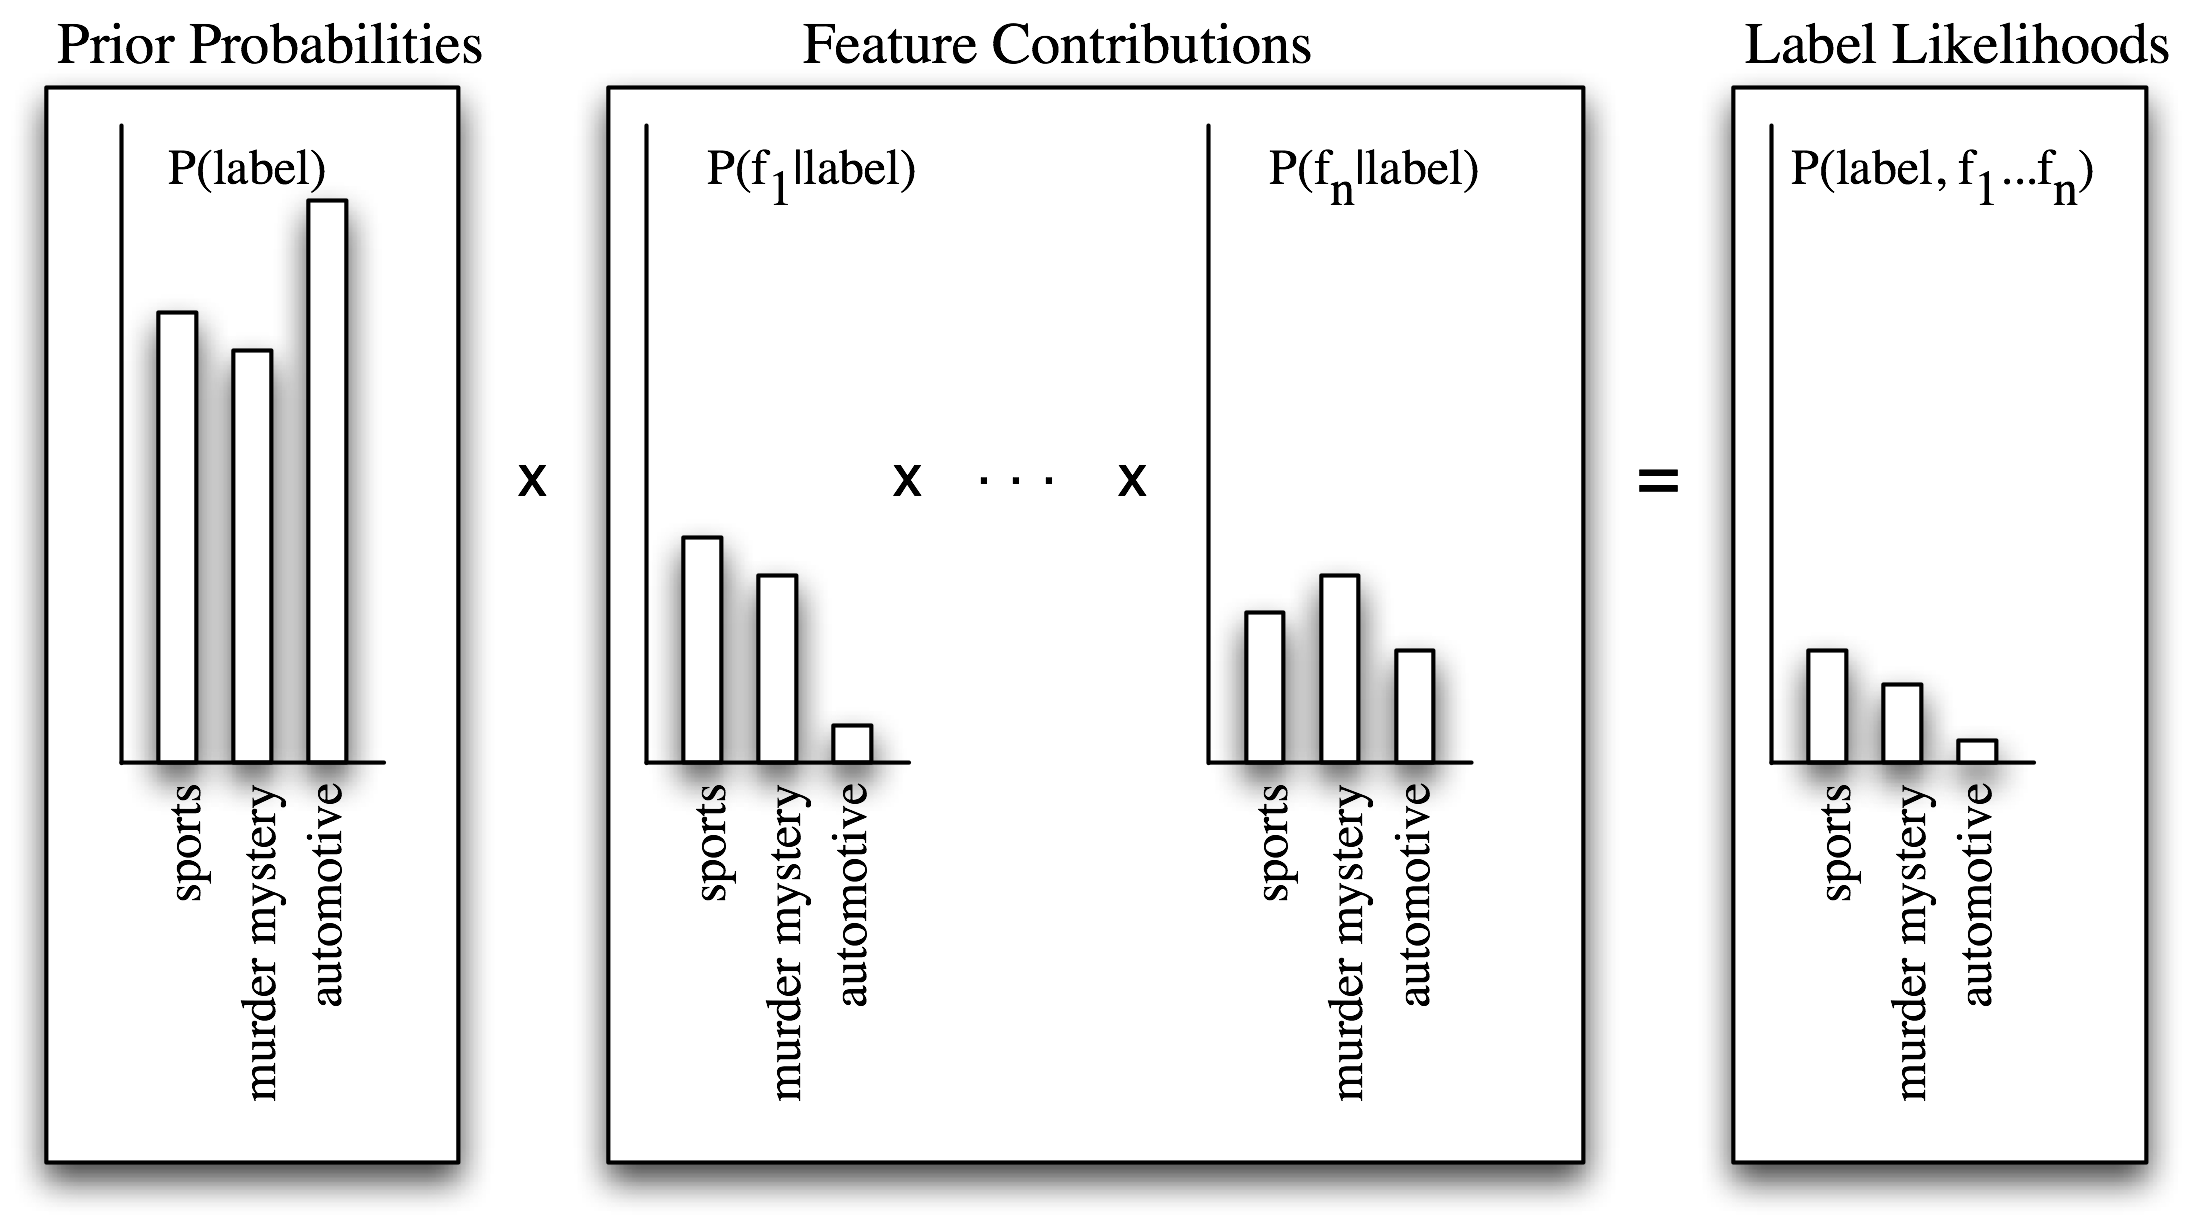
\includegraphics[scale=0.7]{naive_bayes_bargraph.png}
        \caption{Calculating label likelihoods with naive Bayes \parencite{BirdKleinLoper09}}
        \label{fig:Calculating label likelihoods with naive Bayes}
    \end{figure}

    \item Max Entropy
    Like the naive Bayes model, the Maximum Entropy classifier calculates the likelihood of each label for a given input.
    However, Maximum Entropy classifier model leaves it up to the user to decide what combinations of labels and features should receive their own parameters.

\end{itemize}

\section{Related Works}

\parencite{AliCevahir.} describes implementing classification model by chunking the process to predict at every level using the \acl*{KNN} classifier. \parencite{Gupta.20062016}  proposes a distributional semantics representation for predicting the product taxonomies.

\subsection*{Facet Suggestion}


\parencite{Tagliabue.26052020} proposes a machine learning encoder-decoder model architecture that generates the path in catalog taxonomy in real time. This model predicts the best facets - i.e. product categories in real time during type ahead on a eCommerce website search bar. In \parencite{Tagliabue.26052020} work, prediction is based on user personalized model provided with shopping session and user queries. Combining linguistic and behavioral in-session data, narrows down the search results with personalized facet prediction as shown in figure \ref{fig:Personalized facet prediction}. 




\begin{figure}[H]
    \centering    
    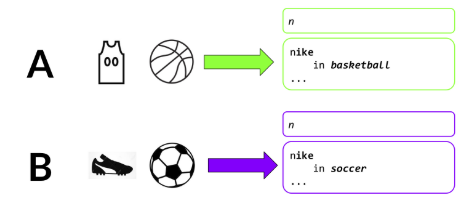
\includegraphics[scale=0.7]{facet2.png}
    \caption{Personalized facet prediction. \parencite{Tagliabue.26052020}}
    \label{fig:Personalized facet prediction}
\end{figure}


\subsection*{Learning to Rank}

Learning to rank is a machine learning algorithm for \acf{IR}. The application of \acf{LTR} model in E-Com is to list most relevant products based on the search query. 

\parencite{KarmakerSantu.2017} uses LambdaMART \parencite{burges2010from} as  \acs{LTR} model as it is well known to work with Web search. As per \parencite{KarmakerSantu.2017}, E-Com search logs contain four prominent relevance feedback signals.

\begin{itemize}
    \item clicks : Computed as the ratio of clicks a product receives for a query and its impressions (number of times shown to the user) for the query.
    \item cart-adds: Computed as the ratio of add-to-carts a product receives for a query and its number of clicks for the query.
    \item orders: Computed as the ratio of orders a product receives for a query and its impressions for the query.
    \item revenue: Computed as the ratio of revenue generated by a product for a query and its impressions for the query.

\end{itemize}

\parencite{KarmakerSantu.2017} proposes an algorithm based on the statistics of feedback signals to rank the relevance of product. 


\subsection*{Conversational commerce}

 Conversational commerce is a way of businesses to interact with customers using chatbots. \parencite{ChrisMessina} inventor of the hashtags, coined the term conversational commerce. In his post, he states that ecommerce will experience transformation, with integration of \acf{AI} specialized in complex task of online shopping and product research.  Conversational commerce offers convenience, personalization and decision support while people are on the go and cannot pay full attention.  
 
 One of the use case of conversational commerce is in the reverse logistics- return and exchange. For example, if the user has ordered and wrong product and would like to return it while being on the go. He may use the chatbot assistance and type "I want to return." The chatbot lists the delivered products list and customer selects the product to be returned. 

%  \begin{figure}
%     \centering
%     \begin{tikzpicture}[node distance=2.5cm, auto,
%         rect/.style={rectangle, draw, text centered},
%         ellipse/.style={ellipse, draw, text centered}
%     ]
%         % Nodes
%         \node [rect] (user) {User};
%         \node [ellipse, below of=user] (order) {Order Wrong Product};
%         \node [rect, below of=order] (chatbot) {Chatbot};
%         \node [rect, below of=chatbot] (list) {List Delivered Products};
%         \node [rect, below of=list] (select) {Select Product to Return};

%         % Arrows
%         \draw [->] (user) -- (order);
%         \draw [->] (order) -- (chatbot);
%         \draw [->] (chatbot) -- (list);
%         \draw [->] (list) -- (select);

%     \end{tikzpicture}
%     \caption{Process of Returning a Wrong Product Using Chatbot}
% \end{figure}
 
Application of knowledge graphs within the e-commerce industry involves the creation of network of information concerning the products. This knowledge graph can serve as the basis for chatbots to provide answers to user queries. 